\documentclass[11pt]{exam}

\usepackage{amsmath, amssymb, multicol}
\usepackage{graphicx}
\usepackage{textcomp}
\usepackage{chessboard}
\usepackage{tikz}
\usepackage{adjustbox}
\usepackage{pdfpages}

\def\d{\displaystyle}
\def\b{\mathbf}
\def\R{\mathbf{R}}
\def\Z{\mathbf{Z}}
\def\st{~:~}
\def\bar{\overline}
\def\inv{^{-1}}
\def\r{2.5pt}
% \def\v{circle (\r)}
\def\vo{node[circle, color=black, fill=white,  inner sep=2pt, minimum size = 17pt, draw]{}}
\newcommand{\vtx}[2]{node[fill,circle,inner sep=0pt, minimum size=4pt,label=#1:#2]{}}
\newcommand{\va}[1]{\vtx{above}{#1}}
\newcommand{\vb}[1]{\vtx{below}{#1}}
\newcommand{\vr}[1]{\vtx{right}{#1}}
\newcommand{\vl}[1]{\vtx{left}{#1}}
\renewcommand{\v}{\vtx{above}{}}

%\pointname{pts}
\pointsinmargin
\marginpointname{pts}
\addpoints
\pagestyle{head}
%\printanswers

\firstpageheader{Math 228}{\bf The Chromatic Function}{Monday, September 24}


\begin{document}

%space for name
%\noindent {\large\bf Name:} \underline{\hspace{2.5in}}
%\vskip 1em
% A \emph{proper vertex coloring} of a graph is a coloring in which no two adjacent vertices are colored the same color.  The \emph{chromatic number} of a graph is the smallest number of colors needed for a proper coloring of the graph.

For any graph $G$, let $P(G,k)$ denote the \emph{number} of proper colorings of $G$ that use up to $k$ colors (that is, we fix a palet of $k$ colors, and each vertex must be one of those $k$ colors, with different colors for adjacent vertices).  So once we have fixed $G$, this will be a function of $k$.

\begin{questions}
  \question For each graph $G$ below, find $P(G, 1)$, $P(G, 2)$, and $P(G,3)$.
  \begin{multicols}{2}
    \begin{center}
      {\tiny
      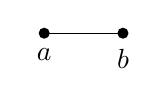
\begin{tikzpicture}
        \draw (0,0) \vb{$a$} -- (1,0) \vb{$b$};
      \end{tikzpicture}
      \vskip 8em
      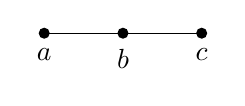
\begin{tikzpicture}
        \draw (0,0) \vb{$a$} -- (1,0) \vb{$b$} -- (2,0) \vb{$c$};
      \end{tikzpicture}
      \vskip 8em
      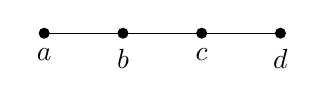
\begin{tikzpicture}
        \draw (0,0) \vb{$a$} -- (1,0) \vb{$b$} -- (2,0) \vb{$c$} -- (3,0) \vb{$d$};
      \end{tikzpicture}
      % \vskip 3em
      }
    \end{center}
    \columnbreak
    {\tiny
    \begin{center}
      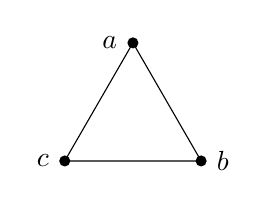
\begin{tikzpicture}
        \draw (90:1) \vl{$a$} -- (210:1) \vl{$c$} -- (-30:1) \vr{$b$} -- cycle;
      \end{tikzpicture}
      \vskip 8em
      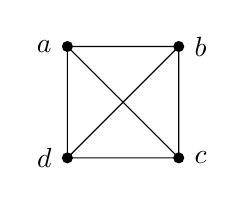
\begin{tikzpicture}
        \draw (45:1) \vr{$b$} -- (-45:1) \vr{$c$} -- (-135:1) \vl{$d$}-- (135:1) \vl{$a$} -- (45:1) -- (-135:1) (-45:1) -- (135:1);
      \end{tikzpicture}
      % \vskip 3em
    \end{center}
    }
  \end{multicols}
  \vfill

  \question Generalize: if $G$ is a path with 4 vertices and 3 edges, what is $P(G,k)$?  What if $G$ is $C_3$ instead?
  \vfill
  \vfill
  \question Use your answers the the previous problem to find $P(G,k)$ for $G = C_4$.  Hint: \emph{any} coloring must either color $a$ and $d$ the same or different.  One of the graphs above allows both of these possibilities, the other has $a$ and $d$ ``the same.''
  \begin{tiny}
    \begin{center}
      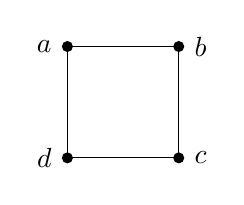
\begin{tikzpicture}
        \draw (45:1) \vr{$b$} -- (-45:1) \vr{$c$} -- (-135:1) \vl{$d$}-- (135:1) \vl{$a$} -- (45:1);
      \end{tikzpicture}
    \end{center}
  \end{tiny}
  \vfill

\end{questions}





\end{document}
